\chapter{Introduction}\label{chap:introduction}

\epigraph{\emph{A program that is used and that, as an implementation of its specification, reflects some other reality, undergoes continuous change or becomes progressively less useful.
The change or decay process continues until it is judged more cost effective to replace the program with a recreated version.}}{--- Meir Lehman}

%\section{The relentless endeavor of software craftmanship}
\lettrine{T}{he} opening quote of this chapter is the first of the five laws of software evolution formulated by Lehman in the late 1970's \cite{Lehman1979}.
The law refers to the fact that all software is designed to operate in a specific environment and to satisfy a specific set of requirements. 
However, every environment, and every requirement, is bound to change eventually, rendering the software obsolete. %, unless it changes accordingly.
Therefore, a constant need of adapting the software and keeping it \emph{relevant} for its stakeholders arises.
This continuous adaptation is a \emph{relentless endeavor} that requires an ever-increasing amount of resources and, over time, destabilises the sustainability of a software project.

A software project is \emph{sustainable} if the project owner is capable of applying whatever valuable change they ought to make, in a timely fashion \cite{Winters2020}.
However, decisions and implementation choices made early on in the project's lifetime inevitably affect the decisions we have to make in the present, often making them harder.
Over time, as the system grows old, our capability of adapting the software to new requirements and changes in the environment grows narrower, and making changes becomes more expensive.
Eventually, the system becomes \emph{unsustainable} and the second part of Lehman's first law of software evolution comes into play.
In other words, a system that is unsustainable is a system that is \emph{poorly maintainable} -- e.g. it is hard to fix bugs -- and with \emph{limited capabilities} to evolve -- e.g. it is difficult to implement new functionality. 

In 1992, Ward Cunningham cleverly adapted and reframed these concepts under the term \emph{technical debt} \cite{Cunningham1992}. 
Since then, technical debt has gained a lot of traction among both practitioners and researchers alike, as it concerns a problem that every non-trivial software system suffers from. 
Over the years, several studies have made great progress in identifying the causes and effects of technical debt \cite{Brown2010,Kruchten2012}.
A comparable amount of effort was also spent in designing and developing strategies and techniques to \emph{manage} TD \cite{Li2015} in order to aid decision-makers. 
Similarly, several tools were developed to automatically \emph{measure} TD using source code as input \cite{Avgeriou2021}, or \emph{track} it manually \cite{Martini2016}.

Technical debt can materialise into various forms, ranging from source code violations \cite{Letouzey2012,Curtis2012} and design level flaws \cite{Marinescu2012} to high-level decisions made at the architectural level \cite{Ernst2015,Yli-Huumo2014}. One form of such architectural decisions are architectural smells (AS); they are defined as a \emph{``commonly (although not always intentionally) used architectural decisions that negatively impact system quality} \cite{Garcia2009} and have gained a lot of attention from researchers over the past years \cite{Verdecchia2018}.
AS contribute to the degradation of a software project's maintainability, and since they involve high-level artefacts, their impact is mostly perceived on the long term. 
%Although existing literature has devoted a considerable amount of effort to study AS \cite{Mo2015,Le2016,Arcelli2016}, our understanding of AS is still incomplete.
%This dissertation aims at improving the current state of the art concerning our understanding of AS by answering questions such as: \emph{how are AS introduced?; how do AS evolve?; and, what is their impact on software maintenance (i.e. technical debt)?}

The fundamental proposition of this thesis is that a better understanding of AS will allow software practitioners to better manage technical debt, thus making software maintainability more cost effective, which slows down the decaying process mentioned by Lehman's first law of software evolution and defers the replacement of the software.

In the upcoming sections, I will introduce the concepts of technical debt and architectural smells in further detail, as these are the \emph{leitmotif} of this dissertation.
I will also decompose the research problem addressed in this thesis into multiple research questions and explain the methodology used to answer them.


\section{Technical Debt}
\subsection{History, definitions, and types}
In 1992, Cunningham first introduced the concept of \emph{technical debt} (TD) \cite{Cunningham1992}. 
The term was coined to indicate the necessity of releasing software that, may work perfectly, but does not meet the criteria of long-term sustainable software. 
Cunningham himself calls this an \emph{``unmasterable program''} that is \emph{``dangerous''} unless the \emph{debt} is repaid.
Unfortunately, TD repayment is not always feasible, as software practitioners have to work with limited time and budget, resulting in most of TD not being repaid \cite{Digkas2018}.
The time spent on not-quite-right code counts as \emph{interest} on that debt \cite{Cunningham1992}, making software projects more expensive to maintain.
Technical debt is a powerful metaphor that, essentially, conveys the importance of sustainable software -- and of Lehman's first law of software evolution -- in terms that are easy to understand and communicate to others. 


A modern definition of TD is the following: 
%\emph{TD reflects the technical compromises that software practitioners make in order to achieve a short-term advantage at the expense of creating a technical context that increases complexity and cost in the long-term} 
\emph{``in software-intensive systems, technical debt is a collection of design or implementation constructs that are expedient in the short term, but set up a technical context that can make future changes more costly or impossible. Technical debt presents an actual or contingent liability whose impact is limited to internal system qualities, primarily maintainability and evolvability''}\cite{Avgeriou2016}. 
Hence, an organization can get into debt and, as long as it is aware of the debt and is planning to repay it in the medium-term period, use it as leverage to temporarily increase productivity.
However, if the organization is not aware that it is accruing TD, or does not repay it on time, the amount of interest may become too high, causing the failure of the project due to the huge cost of implementing changes.

During the course of the years, the metaphor has been extended by the research community and has assumed a wider meaning, engulfing several aspects of the software development process like architecture, design, requirements, testing and documentation \cite{Brown2010}.
The current literature has explored the concept in breadth and depth and has proposed and analyzed multiple taxonomies and types of TD.
A common way of categorising TD is by the type of artefacts it affects. Using this approach, Li et al. \cite{Li2015} identified several different types of TD, namely \emph{Requirements TD}, \emph{Architectural TD}, \emph{Design TD}, \emph{Code TD}, \emph{Test TD}, \emph{Build TD}, \emph{Documentation TD}, \emph{Infrastructure TD}, and \emph{Versioning TD}.

In this thesis, I will mostly focus on \emph{Architectural TD} (ATD), the type of TD that affects the architecture of a software.
Examples of ATD are architectural violations (e.g. the implemented architecture is not compliant with a set of predefined architectural rules), poor application of well-known architectural patterns, early architectural decisions that had unexpected trade-offs, or architectural smells.
As aforementioned, this dissertation is centered around this last form of ATD, that is architectural smells.

\subsection{Metaphor's weaknesses and limitations}
The use of the TD metaphor to describe software issues has received some criticism from the research community too.
One of the major shortcomings of the metaphor, according to Schmid \cite{Schmid2013}, is the lack of a standard unit of measurement and the difficulty to measure it because of the fuzzy boundaries of the different TD components.
Moreover, still according to Schmid \cite{Schmid2013}, not all TD is \textit{effective} TD, but it can also be \textit{potential} TD, since it is not sure if there will be any interest to be paid on that debt.
This may be the case when some specific code will never have to be modified again, hence no interest will ever be paid on such code; as if it had no debt.
Schmid also argues that the more detailed the effect of TD taken into account, the higher its estimation gets: adding up individual contributions to TD will result in counting the same underlying cost multiple times, leading to an exaggerated value of TD \cite{Schmid2013}.

Other studies point out that the metaphor may encourage the detrimental behaviour of introducing debt thinking that a faster delivery can be achieved, without any drawbacks. This is favoured by the fact that, in some cases, the people who take the debt are not necessarily the same who pay it back \cite{Allman2012}.


\section{Architectural smells}
The term \emph{architectural smell} (AS) was initially introduced by Lippert and Roock in 2006 \cite{Lippert2006} to refer to violations of recognised design principles (such as the ones defined by Martin \cite{Martin2018}) that result in undesired dependencies, overblown size, and excessive coupling \cite{Garcia2009}.
Alternatively, architectural smells can be seen as error-prone or change-prone design spots that hinder software maintainability at an architectural level \cite{Mo2015}.
It is important to note, however, that architectural smells are an \emph{indication} that something may be problematic, but they do not necessarily result in problems.

This definition of architectural smells may sound very similar to the definition of \emph{code smells} provided by Kent Beck\footnote{Read \url{https://wiki.c2.com/?CodeSmell} for more info.}. 
However, there is a clear distinction between the two: architectural smells involve multiple classes, packages, architectural layers, or even sub-systems\footnote{From hereon collectively referred to as \emph{elements}.} \cite{Lippert2006}, whereas code smells (CS) arise at line of code, method, or class level \cite{Fowler2002}. 
This means that architectural smells, contrary to code smells, require \emph{large refactorings} in order to be removed from a system \cite{Lippert2006}.
Therefore, given the different scope and granularity, architectural smells and code smells are considered two different categories \cite{Sharma2020}.
In this regard, there exists empirical evidence supporting the difference between the two categories of smells \cite{Arcelli2019}.

Architectural smells can be of different types, with each type having its own definition and implications for the maintainability and evolvability of the affected elements \cite{Azadi2019}.
An architectural smell type can have multiple instances affecting a system, with each instance having a different severity (more on this in Chapter \ref{...}).
An example of an architectural smell type is \emph{Cyclic Dependency}, which arises when a set of elements (e.g. classes, or packages) depend on each other in a cycle.

The architectural smell types that are of interest to this PhD project are \emph{Cyclic Dependency (CD), Hublike Dependency (HL), God Component (GC), and Unstable Dependency (UD)}.
I opted to focus on these four types of AS because, while they are some of the most prominent AS in the literature, there are several important aspects that were not yet investigated. These are extensively elaborated in Section \ref{sec:intro:problem-statement}.
The definitions of each AS type will be given in Chapter \ref{...}.

%\subsection{Why smells over existing metric?}
% TODO?

\section{The project SDK4ED and Arcan}
This PhD project was conducted in the context of the SDK4ED project, a project funded by the European Union under the Horizon 2020 programme.

The vision of SDK4ED is to minimize the cost, the development time and the complexity of low-energy software development projects, by providing tools for automatic optimisation of multiple quality requirements, such as Technical debt, Energy efficiency, Dependability (i.e. Reliability, Availability, and Security) and Performance. 
One of the topics on which the project has innovated, is researching and developing tools to identify the \textit{trade-offs} between runtime and design-time software quality attributes at multiple levels of abstractions (code, design, and architecture).
In this regard, our study investigates specifically the interaction between Technical debt (i.e. Maintainability) and Reliability, a design-time and a runtime quality attribute, respectively. Further details on the project is available on its website\footnote{Browse \url{https://sdk4ed.eu/}.}.

As part of the SDK4ED project, I also contributed to the open source version of \textsc{Arcan}, a tool to automatically detect AS in a system, by adding support for Java source code, support for Git to do evolution analyses, and the detection of the God Component smell.
\textsc{Arcan} will be fully introduced in Section \ref{...}.

\section{Research design}\label{sec:intro:research-design}
\subsection{Problem statement}\label{sec:intro:problem-statement}
Architectural smells management can bring a lot of long-term advantages to practitioners.
However, this begs the following question: what does AS management mean exactly? 
An oversimplified definition would summarise AS management as: (1) \emph{identify} what elements in the system are affected by AS; (2) \emph{quantify} the impact of each smell on the development activities (both maintenance and evolution) in order to determine the urgency to refactor; (3) \emph{make a decision} on whether to keep the smell (i.e. let it accrue interest) or refactor it (i.e. pay back the debt); and finally (4) \emph{repeat} the whole process regularly.
If done manually, this is a rather resource-consuming process, and, in many cases, practitioners have a limited amount of resources they can invest on TD management, in general.

The current research landscape contains plenty of studies that focus on the first phase of AS management: \emph{identification}.
Indeed, the early research work on architectural smells focused on identifying new types of smells, theoretically defining them, proposing detection rules, and finally describing their impact on software maintenance from a theoretical point of view \cite{Lippert2006,Garcia2009,Mo2015,Le2016,Arcelli2016}.
Eventually, tools for automatic detection of AS were proposed, by both academia and industry \cite{Avgeriou2021,Khomyakov2020}, and AS management became a more feasible option for many practitioners that could not afford to do a manual assessment.

Unfortunately, the remaining phases of AS management -- i.e. \emph{quantification} and \emph{decision-making} -- are not as mature as the \emph{identification} phase.
This means that practitioners have the means to identify the AS affecting a system, but there is a limited understanding and tool support for the remaining phases of AS management.
The lack of research in these three areas severely limits the options at the disposal of practitioners, who have to rely on intuition and experience in order make refactoring decisions.

%TODO add what is exactly msising from phases 2 and 3.
%TODO check Jies thesis

The problem is summarised by the following statement:
\begin{quote}\itshape
    ``The detection of the architectural smells alone is not sufficient for practitioners to take informed TD management decisions.
    Practitioners need to understand what lead to the introduction of a smell, the impact of the smell on the system, the available prioritisation strategies, and the amount of TD each instance amounts to.''
    %``Existing literature on architectural smells does not document how AS are introduced, how long they persist, and how software practitioners are impacted by AS. 
    %This limits existing implementations of a fully-automated, data-driven approach to manage the technical debt generated by architectural smells.''
\end{quote}

\subsection{Design science as research methodology}
The research project that this dissertation is based on adopts the design science framework, as developed by Wieringa \cite{Wieringa2014} and depicted in Figure \ref{fig:design-science}.
Design science is the \emph{design} and \emph{investigation} of artefacts (e.g. a software component, a method, a service, an organisation, etc.) in context \cite{Wieringa2014}.
\emph{Design} refers to allowing the design of an artefact that improves a problem context, namely, that solves a \emph{design problem}. 
\emph{Investigation} refers to allowing to answer \emph{knowledge questions} about the artefact in context.

Design problems call for a change in the real world; in contrast, knowledge questions ask for knowledge about the real world.
The distinction between design problems and knowledge questions is often confusing, as design problems can be formulated to look like knowledge questions.
Figure \ref{fig:design-science} can help us distinguish these: if the question asks  \emph{about a solution} to a problem, then it is a design problem; if it seeks knowledge \emph{about the world}, then it is a knowledge question.

A concrete example of design science is Software Engineering itself \cite{Wieringa2014}.
Software Engineering is a design science that seeks to understand and solve the problems of creating and maintaining software to achieve the stakeholders' goals.

A concrete example of a design problem is: \emph{design an approach to measure technical debt principal generated by architectural smells.}
A concrete example of a knowledge question is: \emph{how accurate is such an approach?}

\begin{figure}
    \centering
    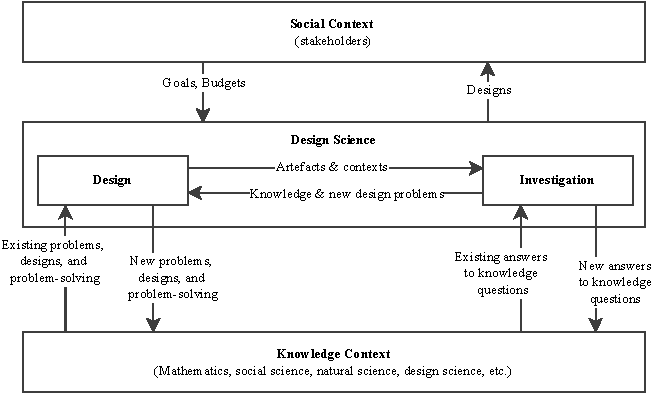
\includegraphics[width=.9\textwidth]{c1/design-science-diagram.pdf}
    \caption{The framework for design science proposed by Wieringa \cite{Wieringa2014}.}\label{fig:design-science}
\end{figure}

Design science is an iterative process where a researcher analyses a design problem, identifies a solution, evaluates the solution, and, if the solution is not satisfactory, they start over. 
The analysis of the design problem and its evaluation are referred to as design cycle.
Iterations through the design cycle may uncover aspects of the original design problem that were initially unknown.
The evaluation process also allows for additional design problems or knowledge questions to emerge.

These characteristics make the design science framework suitable for describing long-term research such as PhD projects.
Indeed, a PhD project starts with an initial problem statement, that leads to new design problems to which the researcher tries to identify a solution by posing new knowledge questions, which in turn might uncover new design problems, and the cycle repeats until a design solution is found for the original problem.

\subsection{Problem decomposition}
This section elaborates on how the research project presented in this thesis is framed into the design science framework. 
Figure \ref{fig:intro:problem-decomposition} decomposes the problem statement introduced in Section \ref{sec:intro:problem-statement} into design problems and knowledge questions.
The different colors and arrows are to be read as follows: light grey boxes refer to design problems; yellow boxes refer to knowledge questions; thin arrows represent decomposition; whereas thick arrows represent sequence.
In the remainder of this section, I will use the term \emph{research question} (RQ) to refer to both design problems and knowledge questions.
Research questions are numbered to easily refer to them, and, with the exception of RQ1, decomposed into multiple sub-RQs that are labelled with letters.

\begin{figure}
    \centering
    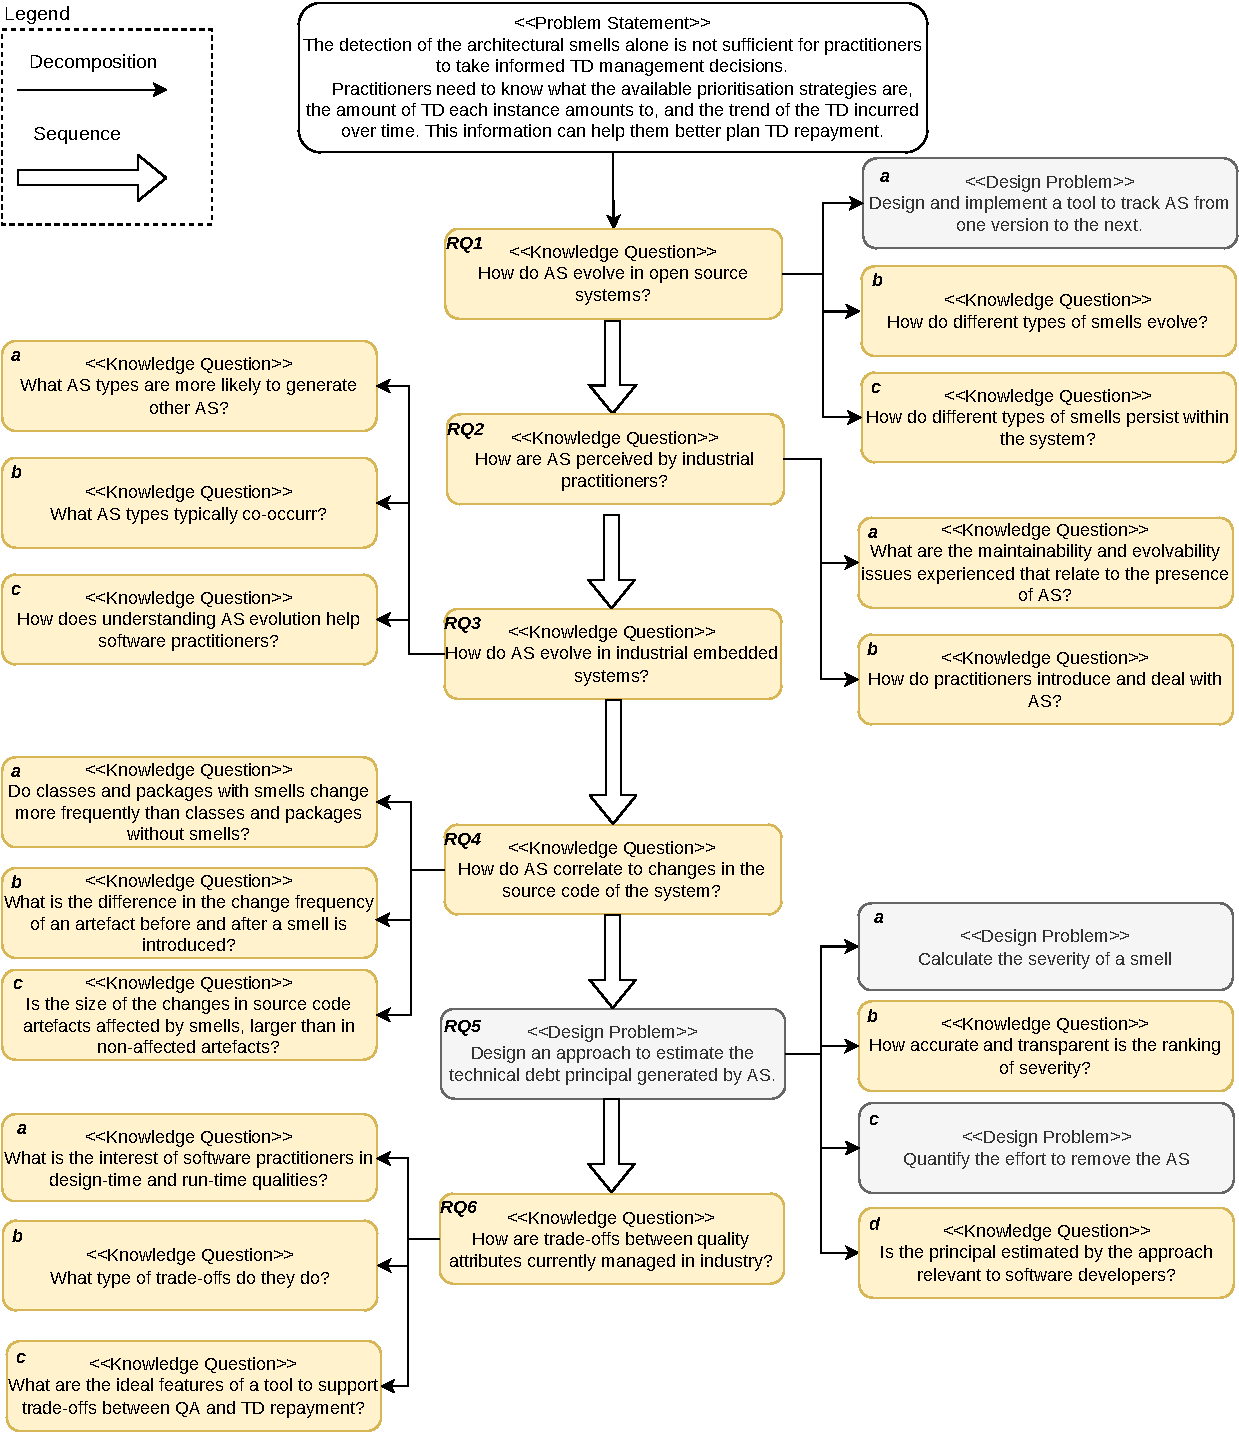
\includegraphics[width=\textwidth]{c1/problem-decomposition.pdf}
    \caption{A caption}\label{fig:intro:problem-decomposition}
\end{figure}

However, there are still three important research threads that are either incomplete or not investigated at all:
\begin{enumerate}
    \item There are no specific details on how individual architectural smell instances evolve over time. This means that it is not clear how architectural smells are \emph{introduced}, how long they \emph{persist} within the system, and whether any TD interest is \emph{paid} on the components affected by architectural smells; 
    
    \item No studies investigate how architectural smells are \emph{perceived} by practitioners. This means that there is little to no empirical evidence on how architectural smells concretely affect the work of software developers and architects;
    
    \item Only a few studies investigate the possibility to \emph{estimate} the amount of technical debt principal generated by architectural smells, but these approaches either lack an industrial validation or use limited approaches to estimate it. 
\end{enumerate}
If architectural smells are to be used by practitioners to manage TD, these three research areas are of paramount importance in order to achieve that.

%Subsequently, researchers moved on to study how smells impact software maintenance in open source systems \cite{Choudhary2016,Xiao2016,Le2018}, study their interaction with other types of smells \cite{Sharma2017,Arcelli2019}, and even predict their introduction in future releases \cite{Arcelli2019b}.
%All of these studies offer a great insight into the theoretical nature of architectural smells, and some of them even provide limited evidence to support whether the hypothesized negative effects on software maintenance are detectable in real world systems.

\subsection{Mapping empirical methods to the RQs}

\subsection{Overview of this dissertation}

